\documentclass[tikz,border=4pt]{standalone}
\usepackage{pgfplots}
\pgfplotsset{compat=1.18}
\usepgfplotslibrary{fillbetween}
\usetikzlibrary{arrows.meta,positioning,calc,shapes.geometric}
\begin{document}
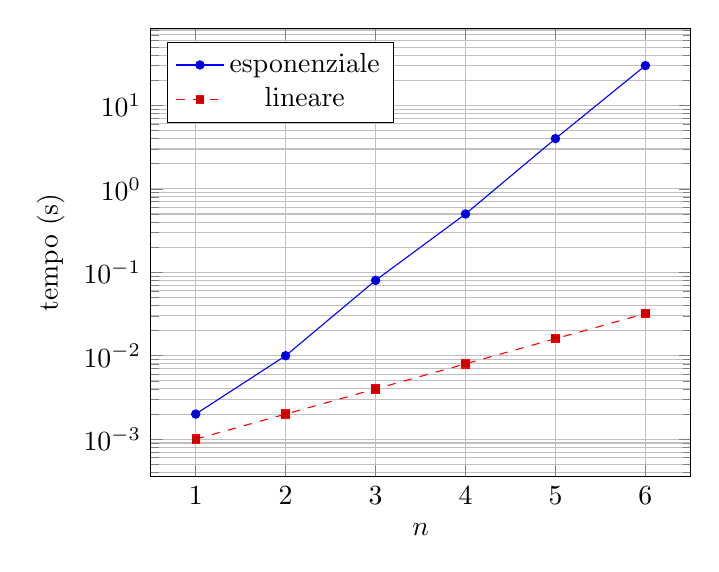
\begin{tikzpicture}
  \begin{semilogyaxis}[xlabel={$n$}, ylabel={tempo (s)}, grid=both, legend pos=north west, mark size=1.5pt]
    \addplot coordinates {(1,0.002) (2,0.01) (3,0.08) (4,0.5) (5,4) (6,30)};
    \addplot+[dashed] coordinates {(1,0.001) (2,0.002) (3,0.004) (4,0.008) (5,0.016) (6,0.032)};
    \legend{esponenziale, lineare}
  \end{semilogyaxis}
\end{tikzpicture}
\end{document}
